\section{Background Subtraction and Person Isolation}
\label{background subtraction and person isolation}
In order to create a point cloud of a person, the tool kit must be able to isolate the person being scanned from the background environment. This is a well researched problem and is an issue for many applications in the computer vision field. Background subtraction is a commonly used class of techniques for segmenting out objects of interest in a scene for applications such as surveillance \cite{McIvor2000}. Even though many background subtraction algorithms have been proposed in the literature, the problem of identifying moving objects in complex environment is still far from being completely solved \cite{Cheung2007}.\\

There are many algorithms for isolating objects and relatively few, to no, algorithms specifically designed to isolate only a person. Therefore, research focused on generic isolation algorithms.\\

\subsection{General Approaches, Properties and Steps}
A common approach for isolating general objects is to perform background subtraction, which identifies moving objects from the portion of a video frame that differs significantly from a background model \cite{Cheung2007}.
This general approach allows the isolation of non humanoid objects such as cars, but is still worthy of note because any person isolation algorithm must shared some similarities with generic object isolation algorithms.\\

These similarities between the algorithms for object isolation and person isolation are that both must \cite{Cheung2007}:\begin{itemize}
  \item Be robust against changes in illumination
  \item Avoid detecting non-stationary background objects such as swinging leaves
  \item React quickly to changes
\end{itemize}

Approaches to object isolation vary from simple techniques such as frame differencing and adaptive median filtering, to more sophisticated probabilistic modelling techniques. 
While complicated techniques often produce superior performance, experiments \cite{Cheung2007} show that simple techniques such as adaptive median filtering can produce good results with much lower computational complexity.\\

In general, the four major steps in a background subtraction algorithm are preprocessing, background modelling, foreground detection, and data validation.
Preprocessing consists of a collection of simple image processing tasks that change the raw input video into a format that can be processed by subsequent steps and can involve noise reduction and frame size/rate reductions \cite{Cheung2007}\\.

Background modelling uses the new video frame to calculate and update a background model.
This background model provides a statistical description of the entire background scene and can be non-recursive or recursive. 
A non-recursive technique uses a sliding-window approach for background estimation. 
The technique stores a buffer of the previous $L$ video frames, and estimates the background image based on the temporal variation of each pixel within the buffer.
Non-recursive techniques are highly adaptive as they do not depend on the history beyond those frames stored in the buffer \cite{Cheung2007}, which may make the ideal for the tool kit.
On the other hand, the storage requirement can be significant if a large buffer
is needed to cope with slow-moving objects \cite{Cheung2007}, although that should not be a problem for the tool kit. Recursive techniques do not use a buffer but maintain a single background model based on each input frame. As a result, input frames from distant past could have an effect on the current background model \cite{Cheung2007} and hence may not be suitable for the tool kit.\\

Foreground detection then identifies pixels in the video frame that cannot be adequately explained by the background model and outputs them as a binary candidate foreground mask. 
Data validation examines the candidate mask and attempt to reduce false-positive or false-negative regions and eliminates those pixels that do not correspond to actual moving objects, and outputs the final foreground mask \cite{Cheung2007}.\\

\subsection{Specific Algorithms}
This section will give an overview of several background isolation algorithms in preparation for comparisons to be conducted in Section \ref{research: person isolation: comparisons}.\\

\subsubsection{Frame Differencing}
\subsubsection{Approximate Median Filtering} \subsubsection{Kalman Filtering}
\subsubsection{Median Filtering}
\subsubsection{Mixture of Gaussian}
\subsubsection{Running Gaussian average}
, where,
for
each
pixel,
the
classification is
just
a thresholded difference and the
background model update adapts
just
one
or
two
parameters.
\subsubsection{Temporal Median Filter}
\subsubsection{Kernel density estimation (KDE)}
\subsubsection{Sequential KD approximation}
\subsubsection{Cooccurence of image variations}
\subsubsection{Eigenbackgrounds}

\subsection{Comparisons of Algorithms}
\label{research: person isolation: comparisons}

\subsubsection{Comparing Frame Differencing, Median, Kalman and Gaussian Filtering.}
Cheung \cite{Cheung2007} conducted a study into the relative effectivenesses of Frame differencing (FD), Approximate median filtering (AMF), Kalman filtering (KF), Median filtering (MF) and Mixture of Gaussian (MoG). In Cheung's experiments, the aim was to isolate vehicles on the road, rather than people. The initial parameters of each filter is shown in Figure \ref{fig:background modelling schemes tested and their parameters}.\\

\begin{figure}[h]
\begin{center}
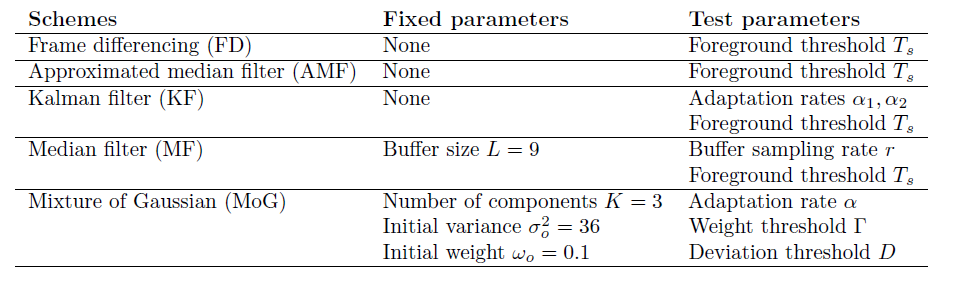
\includegraphics[scale=0.4]{./research/schemes} 
\end{center}
\caption{Background modelling schemes tested and their parameters \cite{Cheung2007}.}
\label{fig:background modelling schemes tested and their parameters}
\end{figure}

Cheung \cite{Cheung2007} selected four publicly-available urban traffic video sequences from the website maintained by KOGS/IAKS Universitaet Karlsruhey. A sample frame from each sequence is shown in Figure \ref{fig:sample frames from the four test sequences: Bright, Fog, Snow and Busy}.\\ 

\begin{figure}[h]
\begin{center}
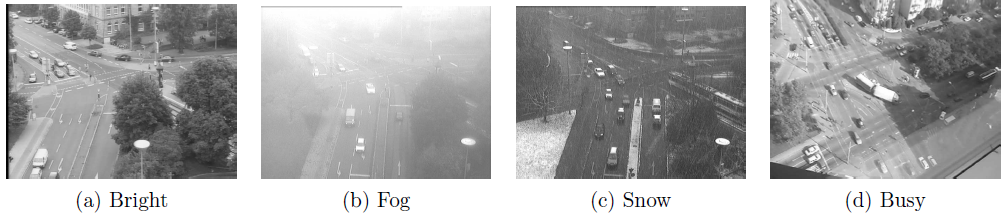
\includegraphics[scale=0.4]{./research/samples} 
\end{center}
\caption{Sample frames from the four test sequences: Bright, Fog, Snow and Busy. \cite{Cheung2007}.}
\label{fig:sample frames from the four test sequences: Bright, Fog, Snow and Busy}
\end{figure}

In Cheung's experiments \cite{Cheung2007} MoG achieved the best precision, MF was a very close second, followed by AMF and KF. FD was significantly worse than all the other schemes. Even though AMF performed worse than MoG and MF, it produced a good performance with an extremely simple implementation. The only drawback of AMF was that it adapts slowly toward a large change in background \cite{Cheung2007}. However this is not expected to be a problem for the tool kit as the should not be any large changes in the background of a doctor's office.\\

Visually, KF produced the worst foreground masks among all the schemes. Even with a large foreground threshold and slow adapting rates. as a result, it typically left a long trail after a moving object \cite{Cheung2007}. Slow updating may be an issue if the  person is required to move at all during the scan.\\

Such experiments suggest that, at this early stage, Adaptive Mean Filtering may be the way forward.\\

\subsubsection{Comparing Running Gaussian average, Temporal Median Filter, Kernel density estimation, Sequential KD approximation, Cooccurence of image variations and Eigenbackgrounds \cite{Piccardi2004}.}

This section presents a comparative performance analysis based on
speed, memory requirements and accuracy of Running Gaussian average, Temporal Median Filter, Kernel density estimation, Sequential KD approximation (SDKA), Cooccurence of image variations and Eigenbackgrounds isolation algorithms \cite{Piccardi2004}.\\

The fastest amongst the methods reviewed by Piccardi \cite{Piccardi2004} was the Gaussian average, having a time complexity of $O(1)$.
Temporal Median Filter has a similar classification cost, but updating the  model is approximated as linear in the number of samples, $n$, therefore the corresponding complexity is consider $O(n)$. 
Mixture of Gaussians method has $O(m)$ complexity, where $m$ is the number of Gaussian distributions used, typically 3 to 5. 
The KDE model computes its value in the Gaussian kernels centred on the past 
n frames, thus the complexity is $O(n)$, where $n$ is typically as high as 100. 
However, efficient implementation through the Fast Gauss transform can
limit the actual execution time \cite{Elgammal2003}.





The SKDA method has $O(m)$ complexity, where $m$ is the number of modes of
the approximated pdf. 
The precise number depends on the actual data samples.
This value
is
not
set
a
priori
and
depends on the actual data samples. However,
in Han2007
[I
I]
this
was shown
to
vary between
3
and
11
in
a
test
video.
The
complexity
for
the
cooccurrence-of-image-variations
method can be
estimated
as
O(8
*
(n
+
L'
+
L)LW),
where
n
is
accounted
for
searching the nearest neighbours
amongst
the
n
variations,
L'
is
the estimated cost
for
computing the interpolation
coefficients,
and
L,
that for
applying
them to
the current block; amongst
these,
the
dominant cost
is either
n
or
L'.
The
I?
denominator
spreads the cost
over
the pixels
in
a block. However,
the
reader should
be
reminded
that this
method works
at
block instead
of
pixel
resolution,
and
that
the
cost
for
updating the
model
has
not
been taken
into
account.
Finally,
the eigenbackground method
has an
estimated
complexity per pixel
of
O(M),
where
M
is
the
number
of
the best eigenvectors. Here
as
well, possible
cc~sts
associated with the model update have not
ben
considered.
Table
1.
Background subtraction methods and perfonnr.nce
analysis
(refer
to
text
for
symbol explanation).
3.2
Memory
requirements
For
some
of
the methods reviewed,
the
memory
complexity
per
pixel
is
the
same
as
the time complexity.
Where
this is intuitive,
we
will
not enter
into details.
The
memory
complexity
for
the cooccurrence-of-image-
variations can
be
estimated
as
O(n&),
where
n
is
the
number
of
variations
in
the
training
model and
K
their
dimension.
Again, the
I?
denominator spreads
the
cost
over
the pixels
in
a block. As the
ratio
&
is
by
definition
largely
less
than
1,
the estimated complexity
tnrns
out
less
than
O(n).
At
classification
time,
the
eigenbackground method requires a
memory
complexity
per pixel
O(M),
with
M
the number
of
the best
eigenvectors. However,
at
training
time the method
requires allocation of
all
the
n
training
images, with
an
O(n)
complexity.
3.3
Accuracy
An
extensive accuracy analysis
is
not
possible
in
the
scope of
this
paper,
as
it
would require agreement on
an
experimental benchmark
or
a complex
theoretical
comparison.
Here we
limit
the discussion
to
analyse the
main
model features
and
categorise
each
approach
as
providing
limited,
intermediate,
or
high
(L,
M,
H)
accuracy.
The methods with a background model based
on
a
single scalar
value can guarantee adaptation
to
slow
illumination changes,
hut
cannot cope
with
multi-valued
background
distributions.
As such, they will
be
prone
to
errors
whenever those
situations arise.
However,
if
such
errors
connect
into relatively
small blobs, they can
be
removed
from
the
classified
image by an adequate
size
filter.
Moreover, post-processing based on foreground
object
classification
and
tracking can always recover
errors
performed
at
the background subtraction
level.
For the approximation
of
a multimodal
distribution,
both parametric and non-parametric methods have been
applied successfully. Consequently, both the Mixture of
Gaussians and KDE approaches
can model
well
the
background
pdf
in
general
cases.
In
addition,
in
[7]
the
proposed KDE temporal model
is
complemented by a
double
time
scale, spatial
correlation and a combination
of
blind and
selective
update.
These
features are able
to
mitigate
undesired
artefacts
such
as
ghosts
and
deadlocks.
Mean-shift methods can effectively model a multi-
modal
distribution
without the need
for
assuming the
number
of
modes a
priori.
However,
their
computational
cost
is
very high.
In
the
SKDA approach, they
are
used
only
in
an
initial stage.
The
model update
is
provided by
heuristics for
adapting, creating and merging
the
modes.
[I I]
shows
that
SKDA proves a good approximation
of
a
KDE
model.
3103
Examples
of
the accuracy
achievable by
the
method
based
on
the cooccurrence
of
image
variations
can
he
found
in
[12].
Differently
from
the other
methods, this
method works at
block resolution
in
blocks
of
N
x
N
pixels,
thus limiting the accuracy
achievable
at
pixel level.
In
addition, blocks
located
at
the
border
of
different
background
objects
might not exhibit significant
cooccurrence thus
risking
to
be misclassified.
We experimented the eigenbackgronnd
method with
a
training set
with
n
=
20
recent images
and
M
=
3
eigenbackgrounds.
The
quality of
results
was
good
but
seemed
to
significantly
depend on
the images
used
for the
training
set.
When
the current
image
contained a
moving
object
in the
same
position
as
in a
training
image,
the
projection
in
the eigenspace did
not
remove it
completely.
In
[13],
however,
the
authors report
good
results
with
lower
computational load than a Mixture
of
Ganssians
approach.
4
Conclusions
In
this paper, we have presented
a
review
of
the
most
relevant
background
subtraction methods. This
original review allows
the
readers
to
compare
the
methods’ complexity
in
terms
of
speed, memory
requirements
and
accuracy,
and
can
effectively
guide
them
to
select
the best
method
for a
specific
application in
a principled
way.
Amongst
the
methods
reviewed,
simple
methods
such
as
the
nnming
Gaussian average
or
the
median
filter
offer acceptable accuracy
while
achieving
a
high
frame
rate
and
having limited memory requirements.
Methods
such
as
Mixture
of
Ganssians
and
KDE
prove
very
good
model
accuracy. KDE has a high
memory
requirement (in
the order
of
a
100
frames)
which
might prevent easy
implementation
on
low-memory
devices.
SKDA is
an
approximation
of
KDE
which
proves
almost
as
accurate,
but
mitigates
the
memory requirement
by
an
order of
magnitude
and
has
lower time complexity.
Methods
such
as the
cooccurrence
of
image variations and
the
eigenhackgrounds explicitly address
spatial
correlation.
They
both offer
good
accuracy against reasonable
time
and
memory complexity.
However,
practical
implementation
of the cooccurrence
method
imposes a
trade
off with
resolution.
References
[l]
C.
Wren,
A.
Azarhayejani,
T.
Darrell, and
A.P.
Pentland, “Pfinder: real-time tracking
of
the human
body,”
IEEE
Trans.
on
Patfern
Anal.
and
Machine
Infell.,
vol.
19,
no.
7,
pp.
78g785,
1997.
[2]
D.
Koller,
J.
Weber,
T.
Huang,
J.
Ma14
G.
Ogasawara,
B.
Rao,
and
S.
Russell,
“Towards Robust
Automatic
Traffic
Scene Analysis in Real-time”,
Proc.
ICPR’94,
pp.
126-131,Nov.
1994.
[3]
B.P.L.
Lo
and
S.A. Velastin, “Automatic congestion
detection system
for
underground
platforms,” Proc.
ISIMP2001,
pp.
158-161,
May2001.
[4]
R.
Cucchiara,
C.
Grana,
M.
Piccardi,
and A.
Prati,
“Detecting
moving
objects, ghosts,
and shadows
in
video
streams,”
ZEEE
Tram
on
Paftem
Anal.
and
Machine
Infell,,
vol. 25,
no.
10, pp.
1337-1442,2003,
[5] C. Stauffer
and
W.E.L.
Grimson, “Adaptive
background
mixture
models
for real-time tracking,” Proc.
IEEE
CVPR 1999, pp.
24&252,
June
1999.
[6]
P.
Wayne
Power and
J.
A.
Schoonees,
“Understanding
background
mixture
models
for
foreground segmentation”,
Proc.
of
IVCNZ
2002,
pp.
267-271,
Nov.
2002.
[7] A.
Elgammal,
D.
Hanvood,
and
L.S.
Davis,
“Non-
parametric
model
for
background
subtraction,” Proc.
ECCV 2000,
pp.
751-767,
June 2000.
[SI
D.
Comaniciu
and
P.
Meer,
“Mean
shift
a robust
approach
toward
feature space analysis,”
ZEEE
Trans.
on
Paftem
Anal.
and
Machine
Infell.,
vol.
24,
no.
5,
pp.
603-
619,2002.
[9]
D. Comaniciu,
“An
algorithm for data-driven
bandwidth selection,”
ZEEE
Trans.
on
Patfem
Anal.
and
Machine
Intell.,
vol.
25
no.
2
pp.
281-288,2003.
[lo]
M.
Piccardi,
T.
Jan, “Efficient mean-shift
backgonmd subtraction”,
to
appear
in
Proc. of
IEEE 2004
KIP,
Singapore, Oct. 2004.
[ll]
B.
Han,
D. Comaniciu,
and
L.S.
Davis, “Sequential
kemel density approximation
through mode propagation:
applications
to background
modeling,”
Proc.
Asian Conf.
on
Computer
Vision,
Jan.
2004.
[12]
M.
Seki,
T.
Wada,
H.
Fujiwara,
and
K.
Sumi,
“Background
subtraction
based
on
cooccurrence of
image
variations,” Proc.
CVPR
2003, Vol.
2,
pp.
65-72,2003.
[13]
N.M.
Oliver,
B.
Rosario,
and
A.P. Pentland,
“A
Bayesian
computer
vision
system
for modeling human
interactions,”
IEEE Trans.
on
Paftern
Anal. and
Machine
Zntell.,
vol. 22, no.
8,
pp.
831-843,2000.
[14] A.
Elgammal,
R.
Duraiswami,
and
L.
S.
Davis,
“Efficient kernel density estimation using
the
fast
Gauss
transform with applications
to
color
modeling and
tracking,”
ZEEE
Trans. an
Paffem
Anal.
and
Machine
Infell.,
vol.
25,
no. 11, pp.
1499-1504,2003.
3104





